\section{Covers and Hasse Diagrams}
\label{tree:poset:hasse}

We introduce an easy tool to \emph{draw} a poset. A poset has an order that (by definition) has the transitivity property.
We would like to exploit this transitivity property to help us simplify our
drawing. What we could do is only explicitly represent the relations that are
necessary to \emph{communicate} the order. Indeed, we do not need to draw
all the relations. For example if we have a poset $\P = (\S, \le)$ and $x, y, z
\in \S$, writing $x < y$ and $y < z$ would imply $x < z$ which we would not need
to draw.


What we draw is called a Hasse diagram. With this diagram we only draw
relations between any $x$ and $z$ for which there is no $y$ such that $x < y <
z$.
What is drawn in a Hasse diagram is called the \concept{transitive reduction}
of the relation graph and the relations contained in the drawing are called
\concept{cover relations}. Furthermore, if $x < z$ is a cover relation then we
say that $x$ is covered by $z$ or $z$ covers $x$, and we write $x \lessdot z$
or $z \gtrdot x$.


If we take an interval (see earlier definition in \Cref{tree:poset:sub}) $I
= [x, z]$ and $x < z$ is a cover relation then we have that our interval $I$ is
the set of size $2$ containing $x$ and $z$, i.e. $I = \left\{{x, z}\right\}$.
Note that a locally finite poset $\P$ is completely determined by its cover
relations.

In the Hasse diagram we make the convention that if $x < z$ then $z$ is drawn
\emph{above} $x$ (i.e. with a higher vertical coordinate). Examples of such
diagrams are shown in \ref{fig:stanley:3-1}, where all posets (up to
isomorphism) with at most four elements are drawn.


\begin{figure}
	\centering
	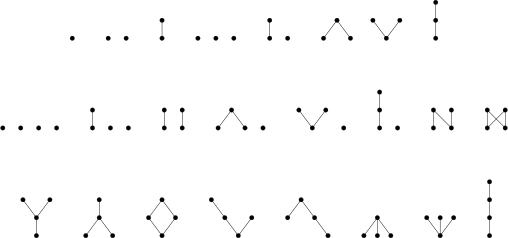
\includegraphics[width=\textwidth]{fig/stanley/3-1}
	\caption{\label{fig:stanley:3-1} The posets with at most four elements,
from \citet*{Stanley:2011:ECV:2124415}.}
\end{figure}


Some care must be taken in \emph{recognizing} posets from their Hasse diagrams.
For instance, 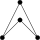
\includegraphics{fig/stanley/3-1:a} is a perfectly
valid Hasse diagram, while not drawn in \ref{fig:stanley:3-1}. This is because
it is another way of drawing one that is already present in
\ref{fig:stanley:3-1} (last one on the second line).
This is what we mean by \emph{up to isomorphism}, \ie that we only consider one
version of isomorphic diagrams. In fact, there are many ways to draw a Hasse
diagram, and some may be better at expressing structural properties of a poset
(e.g. symmetries).


\begin{figure}
	\centering
	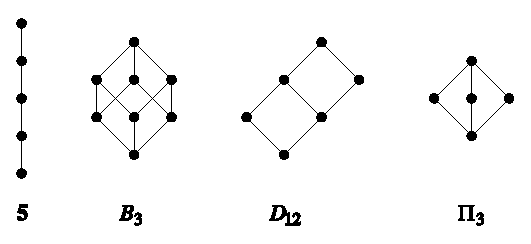
\includegraphics[height=0.2\textheight]{fig/stanley/3-2}
	\caption{\label{fig:stanley:3-2} Some examples of posets, from
\citet*{Stanley:2011:ECV:2124415}.}
\end{figure}


Similarly, the drawing 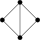
\includegraphics{fig/stanley/3-1:b} is not a Hasse diagram.
This is because we defined earlier that the edges of
the Hasse diagram were the cover relations of the poset.


\ref{fig:stanley:3-2} illustrates the Hasse diagrams of all the posets
considered in \ref{ex:poset:def}.

